\subsection{Untersuchung einzelner Algorithmen}
\label{framework:bechmark:sacabench-construct}

\begin{wrapfigure}{R}{.5\textwidth}
	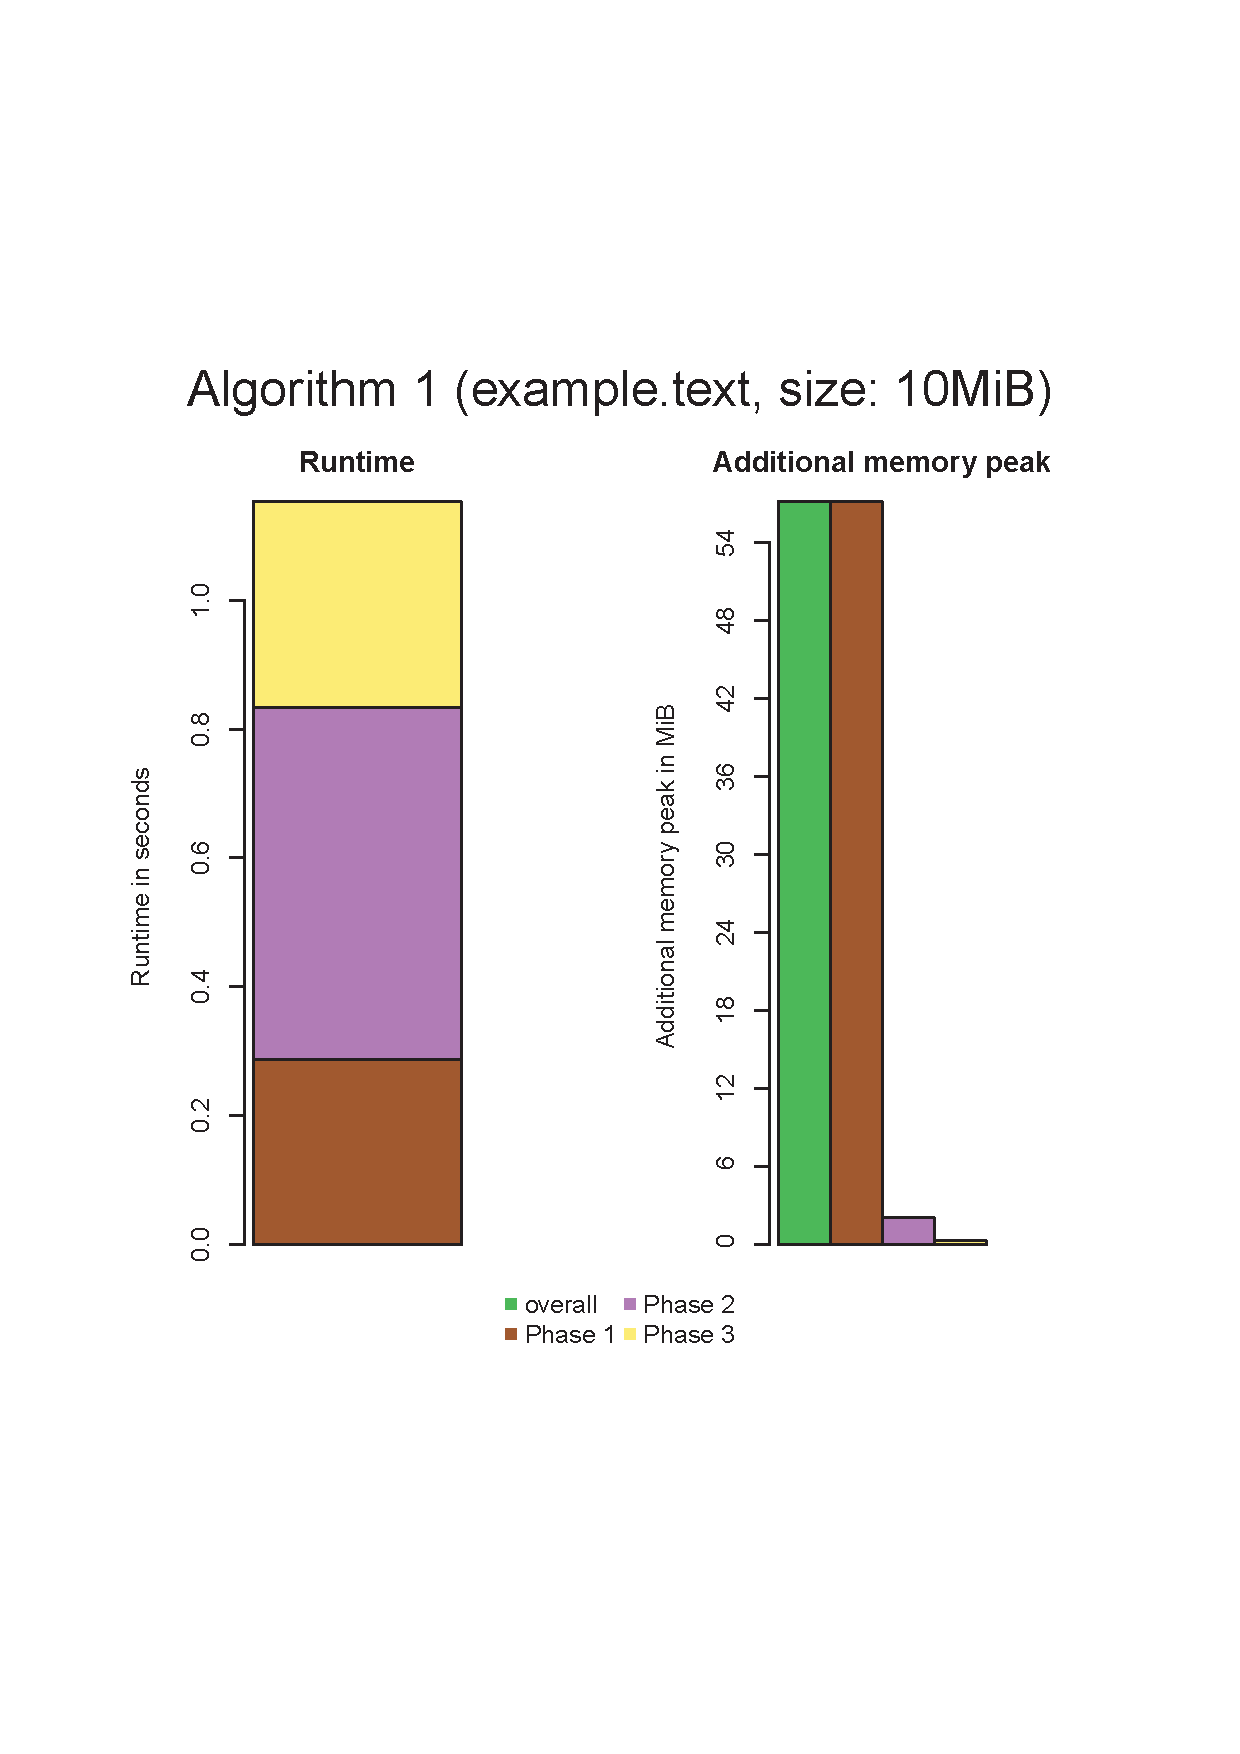
\includegraphics[page = 1, width=.5\textwidth]{kapitel/3_framework/benchmark/sacabench-construct/beispiel_construct.pdf}
	\caption{Messergebniss eines Beispiel-Algorithmus}
	\label{pdf:benchmark:construct}
\end{wrapfigure}


Wird die \texttt{plot}-Option mit dem Befehl \texttt{sacabench construct} ausgeführt, lassen sich einzelne Algorithmen näher untersuchen. Dabei wird die Laufzeit und der maximale Speicherverbrauch des Algorithmus während der Erstellung des Suffix-Arrays gemessen. Zusätzlich gibt es die Möglichkeit, Implementierungen der Algorithmen in Phasen aufzuteilen. Dies ermöglicht eine bessere Übersicht und gegebenenfalls eine schnellere Auffindung von Schwachstellen der eigenen Implementierungen.
Als Ergebnis wird eine zweiseitige \texttt{PDF}-Datei erstellt, die in dem Pfad abgespeichert wird, der hinter der Option \termfont{-b} oder \termfont{-{}-benchmark} angegeben worden ist.

Die \cref{pdf:benchmark:construct} zeigt die erste Seite der \texttt{PDF}-Datei. Dort ist als Überschrift sowohl der Name des Algorithmus als auch der zu untersuchende Text mit dessen Größe angegeben. Die darunter abgebildete Grafik stellt die Messergebnisse dar. Die Grafik ist wiederum in zwei Bereiche aufgeteilt. Auf der linken Seite ist ein gestapeltes Säulendiagramm zu erkennen, das die Laufzeit repräsentiert. Jeder Stapel auf diesem Säulendiagramm entspricht der Laufzeit einer Phase. Die Zeiteinheit, die auf der Y-Achsenbeschriftung niedergeschrieben ist, wird dabei je nach Laufzeit angepasst, sodass die Übersicht gewahrt ist. Auf der rechten Seite befindet sich ein Säulendiagramm, das den Speicherverbrauch widerspiegelt. Auch hierbei stellt jede Säule eine Phase dar. Der Speicherverbrauch wird so gemessen, dass pro Phase jeweils der maximal gemessene Verbrauch des Speichers ohne Berücksichtigung des Ausgangstextes dargestellt ist. Welche Phase zu welchem Stapel, beziehungsweise welcher Säule gehört, ist der Le\-gen\-de, die sich in der Fußzeile der ersten Seite befindet, zu entnehmen.

Auf der zweiten Seite befindet sich eine Auflistung der tech\-nisch\-en Daten des auszuführenden Systems, das sogenannte \texttt{experimental setup}. Dazu gehört der Prozessor mit der zugehörigen Frequenz, sowie die maximale Turbo-Frequenz. Ebenfalls wird die Größe des Ar\-beits\-spei\-chers angezeigt. Zusätzlich wird auch auf dieser Seite erneut der Name und die Größe des Textes angegeben, zu dem das Suffix-Array erstellt worden ist.